% vim: set ts=4 sw=4 smartindent expandtab textwidth=100:

\section{Entity Component System}
Zu Beginn der Implementierung wurde über verschiedene Entity Component Systeme (ECS) recherchiert. Die folgenden Kriterien wurden bei der Auswahl eines passenden ECS berücksichtig. 
\begin{itemize}
	\item Aktive Entwicklung
	\item Datum des letzten Updates
	\item Unterstützte Sprachen
	\item Qualität der Dokumentation
	\item Performance
	\item Unterstützung des Open-Source-Paketmanager vcpkg
\end{itemize}
Bei der Recherche wurden, die folgenden zwei ECS, Flecs und EnTT, in Betracht gezogen. Letztendlich fiel die Wahl auf Flecs, da dieses besser dokumentiert ist und das letzte Update aktueller war. 
Im Anschluss an die Recherche wurde Flecs mit Hilfe von vcpkg eingebunden. Im Laufe des Projekts wurden die Entities Spieler, Pflanzen und Roboter angelegt und erhielten Komponenten, wie beispielsweise Fahr-, Spieler- und Pflanzenkomponente. So enthält zum Beispiel die Positionskomponente Informationen über die Translation, Rotation, Skalierung, Translationsdelta, und Rotationsdelta. Die Pflanzenkomponente speichert, wie viel Wasser sich in der Pflanze befindet und wie viel maximal in den Topf passt. Die Spielerkomponente hat Informationen über den Gamestate, die Kamera, Tastatur und Maus. Des Weiteren wurde die Steuerung der Kamera angepasst. Es wurde die Maus in dem Fenster gefangen, wodurch es nun möglich ist die Kamera zu bewegen, ohne vorher eine Maustaste drücken zu müssen. Zudem wurde die Blickrichtung eingeschränkt, sodass es nicht mehr möglich ist so lange die Maus nach oben zu bewegen, bis das Kamerabild auf dem Kopf steht. Außerdem wurde die Bewegungsgeschwindigkeit des Spielers in Bezug auf das Gehen und Rennen angepasst.
Zudem wurden Systeme, wie das Fahrsystem, Pflanzensystem, Gießsystem und noch viele mehr umgesetzt. Das Pflanzensystem, reduziert bei jedem Aufruf den Wasserstand aller Pflanzen, welches alle Objekte sind, die eine Pflanzenkomponente besitzen. Der Stand kann dabei jedoch nicht negativ werden. Ein weiteres Beispiel ist das „FindePflanzensystem“, welches aus allen Pflanzen diejenige aussucht, welche am wenigsten Wasser hat und diese als neues Ziel festlegt.
Da bei der Implementierung einige Komponenten und Systeme erzeugt werden, ist es entscheidend einen Überblick über diese zu bewahren. Aus diesem Grund wurden im Laufe des Projekts Aufräumarbeiten durchgeführt. Das bedeutet, es wurden Komponenten entfernt, die nicht mehr benötigt wurden. Der Rest wurde in einer Datei zusammengefasst. Das erleichtert zum einen das Einbinden von diesen in anderen Dateien, zum anderen findet man sie leichter. Das Gleiche wurde mit kleinen Systemen gemacht, wie beispielsweise dem AIsystem, dem Pflanzensystem und den beiden Gießsystemen.

\section{Multiagenten System}

\subsection{Sate Machines}

Wir haben noch keine State Machines für den Roboter implementiert, weil der Roboter sich nur in den zwei Zuständen \"Pflanzen gießen\" und \"Mit Spieler reden\" befinden kann. Diese Funktionalität kann über ein einfaches if-else abgedeckt werden und deswegen sind State Machines noch nicht nötig.

\subsection{Behaviour Tree}
Um den Behaviour Tree für den Handlungsablauf des Roboters effizient umzusetzen, wurde die Bibliothek BehaviorTree.CPP genutzt. Diese wurde ausgesucht, da sie vcpkg unterstützt, für C++ entwickelt wurde und alle nötigen Funktionalitäten bietet, ohne zu komplex zu sein. 
Im Falle des Gießroboters gibt es fünf Schritte, die er ausführen muss, um eine Pflanze zu gießen. Zuerst muss eine Pflanze ausgewählt werden, die den geringsten Wasserstand hat. Im Anschluss wird der Weg von der aktuellen Position zu dieser gesucht. Daraufhin fährt der Roboter den Weg ab. Dort angekommen muss er sich noch so drehen, dass sich sein Gießarm über dem Blumentopf befindet, damit am Ende die Pflanze gegossen werden kann und sich ihr Wasserstand erhöht. Alle diese Schritte wurden in dem Behaviour Tree als Blattknoten implementiert. Darüber sitzt ein sogenannter Sequenzknoten, dieser merkt sich welches Blatt als letztes ausgeführt wurde und ob dieses beendet wurde. Wenn es noch nicht fertig ist, wird es im nächsten Schritt erneut aufgerufen. Dies geschieht so lang, bis das Blatt fertig ist. Der Sequenzknoten erhält als Rückmeldung „SUCCES“, oder, wenn das Blatt noch nicht fertig ist, „RUNNING“. Wenn ein Blatt fertig ist, wird das nächste ausgeführt. Wurde jedes Blatt einmal ausgeführt und hat jeweils „SUCCES“ zurückgegeben, so beginnt der Sequenzknoten erneut das erste Blatt aufzurufen.
Die Baumstruktur wird in einem XML-Dokument gespeichert. Die Funktionalität der einzelnen Knoten befindet sich in einer C++ Datei und die Knoten und Blätter werden in einer sogenannten Treefactory erstellt, welche ebenfalls in C++ geschrieben ist.
\subsection{Steering Behaviour}
Auch die Bewegungssteuerung wurde auf Basis des ECS implementiert. Dazu wurden ein Fahrsystem und Komponenten, wie Fahr-, Hindernis-, Pfad- und Positionskomponente, erstellt. Das Fahrsystem untersucht dabei, welcher Bewegungsmodus aktuell ausgewählt ist und passt darauf basierend das Bewegungsverhalten an. Es wird zwischen dem Pfadverfolgen und Drehen unterschieden. Ist Pfadverfolgen aktiviert, so folgt der Roboter einem Pfad, welcher sich in der Pfadkomponente befindet, die dem Entity Roboter zugeordnet wird. Der Pfad ist dabei eine Liste von Wegpunkten, die der Agent abfahren soll. Dazu wird das, wie im Konzeptteil beschriebene Suchverhalten genutzt. Zudem wird, während der Roboter die Punkte abfährt, darauf geachtet, dass er mit keinen Hindernissen kollidiert. Diese sind alle Objekte in der Szene, welche eine Hinderniskomponente haben. In dieser ist der Radius des Gegenstandes oder Spielers gespeichert. Damit das Fahrverhalten des Roboters sichtbar ist, muss die Position in der Positionskomponente nach jedem Durchlauf aktualisiert werden. Das Ausweichverhalten wurde, wie oben erwähnt, implementiert. Das bedeutet, es wird überprüft, ob das Objekt, welches am nächsten zu dem Roboter ist, sich vor dem Agenten befindet. Ist dies der Fall, so wird getestet, ob der Roboter nach dem nächsten Schleifendurchlauf mit diesem kollidiert, wenn ja wird der aktuelle Wegpunkt nach rechts oder links verschoben. Es wird dabei berücksichtigt, bei welcher Verschiebung die Abweichung zum Pfad am geringsten ist. Je nach dem wird der Pfad angepasst. Da der Punkt nun eine neue Position hat, weicht der Roboter dem Hindernis aus.
Soll der Roboter sich drehen, um beispielsweise mit dem Spieler zu reden, oder um eine Pflanze zu gießen, muss in der Fahrkomponente der aktuelle Modus auf Drehen gesetzt werden. In ihr sind zudem Informationen über die Masse, die Höchstgeschwindigkeit, die maximale Lenkkraft und die Größe des Sicherheitsabstandes gespeichert. Bei der Implementierung des Drehverhaltens werden jedoch keine weiteren Punkte bestimmt, die der Agent anschauen soll, sondern der Drehwinkel wird interpoliert. Das bedeutet, dass der Wert für diesen reduziert wird, sodass der Roboter sich unabhängig von der Framerate langsam in die richtige Richtung dreht und zum Schluss korrekt ausgerichtet ist. Alle Objekte, die sich in dem Projekt bewegen sollen, erhalten eine Fahrkomponente, aktuell sind dies die zwei Gießroboter.
Die Bewegungssteuerung hat noch zahlreiche Probleme. Da die Steuerung des Roboters auf einfachen mathematischen Formeln basiert, verfügt der Roboter nur über ein stark eingeschränktes Wissen über die Umgebung. Aus diesem Grund kann er zwar einem Hindernis ausweichen, es wird jedoch dabei immer nur ein Objekt berücksichtigt. Das bedeutet, dass er beispielsweise rechts an einem Hindernis vorbeifährt und damit auf einen Kollisionskurs mit einem anderen Gegenstand gerät, was nicht passiert wäre, wenn er dem ersten Hindernis auf der linken Seite ausgewichen wäre. Hätte der Roboter ein besseres Verständnis über die aktuelle Situation, so könnte er sich besser in der Welt bewegen. Zudem wird bei dem Ausweichverhalten nicht zwischen Objekten unterschieden, die stillstehen, oder sich bewegen. Es könnte passieren, dass er einen Bogen nach rechts fährt, um einem Objekt auszuweichen, dieses sich jedoch so bewegt, dass es trotz Ausweichmanöver immer noch im Weg befindet. Im schlimmsten Fall könnte dieses Hindernis sich aufgrund seiner Bewegung dauerhaft zwischen Roboter und Ziel befinden. In dieser Situation wäre es für ihn mit dem aktuell implementierten Bewegungssystem unmöglich die Pflanze zu erreichen.
Des Weiteren kann auf Grund der Simplizität nicht garantiert werden, dass der Roboter, während er auf eine Pflanze zufährt, nicht auf eine Kreisbahn um diese gelangt. Dies würde geschehen, wenn das Ziel sich links beziehungsweise rechts von dem Roboter befindet und er eine Kurve fahren muss, um es zu erreichen. Wenn die Krümmung der Kurve stärker ist, als der Roboter mit seinem maximalen Lenkwinkel fahren kann, ist es für ihn unmöglich diesen Pfad zu fahren. Im schlimmsten Fall befindet sich das Ziel im Mittelpunkt der Kurve, die der Roboter aktuell fährt und dem maximalen Lenkwinkel entspricht. Dies hätte zur Folge, dass sich der Abstand zur Pflanze nicht verändert und er sie nicht erreichen kann. Das aktuell implementierte Bewegungssystem kann nicht erkennen, ob er auf einer Kreisbahn ist. Daher können auch keine Korrekturzüge ausgeführt werden.
Außerdem ist die Bewegungssteuerung nicht intuitiv, da Eigenschaften wie die Masse des Roboters oder seine maximale Krafteinwirkung diese beeinflussen. Es ist dementsprechend bei der Erstellung neuer Roboter schwierig passende Werte für die Merkmale zu finden, um das gewünschte Fahrverhalten zu erhalten.

Während der Programmierung traten zahlreiche Herausforderungen auf, insbesondere aufgrund der begrenzten Erfahrung mit C++. Zum Beispiel wurde in der Funktion, die das Gießen der Pflanzen steuert, zu Beginn ein Pointer auf die ID des gießenden Roboters genutzt. Allerdings wurde dieser ungültig, sobald der Funktionsaufruf beendet wurde. Dies führte dazu, dass keine Unterscheidung zwischen den beiden Robotern mehr möglich war. Die ID musste aus diesem Grund als Variable vom Typ flecs::id_t gespeichert werden. Ein weiteres Problem entstand bei der Berechnung der Steuervektoren. Dieser zeigte beispielsweise in Richtung minus unendlich, wenn durch Zufall das Ziel die Koordinaten (0,0,0) hatte. 
Zudem wurden verschiedene IDEs verwendet. Das hatte zur Folge, dass Veränderungen, die in einer IDE gemacht wurden zu Fehlern in einer anderen führen konnten. Ein Beispiel hierfür ist die Deaktivierung von Backface Culling in CLion. Wenn nun das Projekt in Visual Studio gestartet wurde, kam es zu einem fehlerhaften Speicheraufruf. Durch sorgfältiges Analysieren und Zusammenarbeiten konnten jedoch viele Probleme im Verlauf des Projekts bewältigt werden. 

\section{Partikelsystem}
Um das Partikelsystem in dem Projekt umzusetzen, wurden zwei neue Komponenten mit zusätzlich zwei weiteren Systemen implementiert. Die Komponenten waren dabei eine Emitter- und eine Partikelkomponente. Die Emitterkomponente enthält Informationen über die Anzahl der Partikel, die pro Iteration erschaffen werden und die relative Position, wo dies geschehen soll. In dem Projekt muss berücksichtigt werden in welche Richtung der Roboter schaut, damit die Wassertropfen an der Stelle erscheinen, wo sich der Arm des Roboters befindet. In der Partikelkomponente wird die sogenannte Lebensdauer gespeichert, die es erlaubt die Tropfen nach einer definierten Zeit verschwinden zu lassen beziehungsweise diese zu entfernen. Das ist von großer Bedeutung, da sonst immer mehr Entities erschaffen werden, was die Performance stark reduzieren würde und im schlimmsten Fall das Programm zum Absturz bringen kann. Das Partikelsystem erschafft Objekte mit einer Partikelkomponente, Geometriekomponente und einer Positionskomponente. Die Geometriekomponente ist dabei wichtig, um den einzelnen Tropfen ein Modell zuzuordnen, anderenfalls wäre der Benutzer nicht in der Lage das Wasser zu sehen. Bei der Erstellung der Entities wird zudem darauf geachtet, dass die Position, an der sie erschaffen werden, leicht variiert. Dadurch entsteht ein breiterer Strahl aus Tropfen, was das Gießen realistischer darstellt. Das zweite System ist das PartikelRemovalSystem. Dieses reduziert bei jeder Iteration den Wert der Lebensdauer aller Tropfen, bis dieser kleiner gleich Null ist. In diesem Fall wird das entsprechende Objekt entfernt.
\section{Navigationssystem}

Um einen Pfad für ein Entity zu finden, muss man dem Entity eine PathRequestComponent mit Start und Ziel hinzufügen. Das Navigationssystem liest die Daten aus dem Request aus, entfernt diesen und fügt stattdessen eine PathComponent mit dem gefundenen Pfad hinzu.

Um einen Pfad von einem Startpunkt zu einem Zielpunkt zu finden, sind drei Schritte nötig. Zuerst muss man die Navigationsnetzpolygone finden, auf denen Start und Ziel liegen. Danach sucht man die Polygone, die Start- und Zielpolygon verbinden, und zum Schluss kann man diese Liste an Polygonen zu einem Pfad aus Punkten umwandeln.

\section{Physiksystem}

Die ECS-Bibliothek Flecs unterstützt Entity Event Listener, sogenannte Observer. Man kann eine Callbackfunktion definieren die gerufen wird, wenn eine Komponente eines Entities hinzugefügt, modifiziert oder entfernt wird. Das Physiksystem nutzt zwei Observer: ein Observer überwacht, wenn eine Physikkomponente zu einem Entity hinzugefügt wird und fügt den enthaltenen Rigidbody auch in die Physikwelt ein. Der zweite Observer wird gerufen, wenn ein Entity aus der Welt entfernt wird, welches eine Physikkomponente besitzt. In dem Fall wird auch der dazugehörige Rigidbody aus der Physikwelt entfernt.

Theoretisch benötigen wir nur die Kollisionserkennung und -auflösung von Bullet. Aber es war deutlich schwerer, diese beiden Funktionen getrennt von der Physiksimulation zu rufen, als die Physikwelt und die ECS-Welt zu synchronisieren. Deswegen funktioniert die Kollisionserkennung und -auflösung jetzt in drei Schritten. Zuerst werden alle Entities mit Physikkomponente und Transformationskomponente gesucht und die Geschwindigkeit und Position der Transformationskomponente auf den Rigidbody der Physikkomponente übertragen. Dann wird die Simulation der Physikwelt mit dem jetzigen Zeitschritt gerufen. Zum Schluss werden die Geschwindigkeit und Position des Rigidbodies wieder in die Transformationskomponente geschrieben.

Die Plattformen, Zäune und Wendeltreppe sind statische Geometrie und zusätzlich noch konkav. Deswegen sind diese mit einem Deiecks-Collider repräsentiert. Dabei wird einfach das 3D-Modell der statischen Geometrie als Collider benutzt.

Alle Entities haben Kapsel-Collider anstatt Zylinder-Collider, da diese an den Dreieckskanten der statischen Geometrie hängen geblieben sind.

\section{Szenen Editor}

Die Assimp-Variante hat nicht funktioniert, weil die Eingriffe zu tief in der Engine vorgenommen werden mussten. Außerdem war das Abstraktionslevel zu gering: wenn man nur Knoten hat, ist es schwer, Entities zu erkennen.

Das Blender Plugin wurde in Python programmiert, und man hat Zugriff auf alle Optionen, auf die man auch im Editor Zugriff hat. Um jetzt die Entities zu exportieren, wird über alle Objekte der Szene iteriert und überprüft, ob diese gelinkt sind. Ist dies der Fall, dann wird die Transformation, der Name und der Name der Modelldatei in eine JSON-Datei geschrieben. Um jetzt auch noch die statische Geometrie zu exportieren, werden alle gelinkten Objekte unsichtbar gemacht, und nur die sichtbaren Modelle werden exportiert. Alle unsichtbaren Objekte werden anschließend wieder sichtbar gemacht, um den Ausgangszustand wieder herzustellen.

In CrossForge wird dann die JSON-Datei geladen und für jeden Eintrag ein entsprechendes Entity zur Welt hinzugefügt.

\section{Dialogsystem}

Die gesamte Implementierung des Dialogsystems haben wir (Lisa und Sophie) im Pair-Coding übernommen. 

\subsection{Imgui}

Die Bibliothek für Imgui konnte über vcpkg recht schnell und einfach in das Projekt eingebunden werden. Zur Erzeugung von Dialogfenstern erstellen wir mit Imgui Frames, in denen oben der aktuelle Text des Dialogs angezeigt wird und unten die möglichen Antworten als Buttons. Wir nutzen außerdem einige Style-Anpassungen, um den Dialog etwas anschaulicher für den Nutzer zu gestalten, sodass z.B. das Fenster immer im Viewport zentriert ist.

\subsection{JsonCpp}

Ähnlich wie Imgui konnten wir auch JsonCpp über vcpkg einbinden. Mithilfe dieser Bibliothek können wir dann den Dialoggraphen initialisieren. Dafür sollten die Json-Dateien die gleiche Baumstruktur aufweisen, wie der Dialoggraph selbst. Über JsonCpp werden die Informationen aus der Datei gelesen und gespeichert, sodass sie dann weiter genutzt werden können, um den Dialoggraph zu füllen.

\subsection{Dialoggraph}

Den Dialoggraph haben wir so wie im Konzeptteil beschrieben implementiert. In einer dafür erstellten Klasse werden die zuvor genannten Daten gespeichert: der Dialogtext, ein Boolean für die Unterscheidung zwischen Roboter und Spieler und die möglichen Antworten. Zusätzlich gibt es noch eine Funktion, die die Initialisierung des Baumes umsetzt und eine Funktion für das Ersetzen der Strings mithilfe der Dialogmap.

\subsection{Dialogmap}

Mit der implementierten Dialogmap kann eine Funktion aufgerufen werden, die den Name einer Pflanze zurückgibt. Der Rückgabewert dieser Funktion ist allerdings statisch festgelegt, da zum Zeitpunkt der Abgabe das Dialogsystem noch nicht in das ECS eingebunden ist. Diese Integration wäre aber notwendig um die Positionen von Roboter und Spieler zu ermitteln, die gebraucht werden um zu bestimmen welcher Pflanzenname zurückgegeben werden soll. Auch die Pflanzennamen selbst sind im ECS gespeichert, weshalb ein Zugriff darauf vom Dialogsystem aus aktuell nicht möglich ist.  
Weitere Funktionalitäten der Dialogmap, wie Eventhandling sind ebenfalls noch nicht implementiert.

\section{Modelle und Szene}

Wie im Konzept bereits erläutert, wurde ein beträchtlicher Teil der Anfangsphase für die Konzeptentwicklung aufgewendet. Darüber hinaus erforderte die Einarbeitung in Blender eine gewisse Zeit. Die Modellierung aller Objekte musste aufgrund verschiedener Herausforderungen mehrfach überarbeitet werden, darunter Unklarheiten im Design, zu viele Polygone aufgrund detaillierter Elemente oder inkorrekter Vorgehensweisen, usw.
\begin{figure}[H]
	\begin{subfigure}{0.5\textwidth}
		\centering
		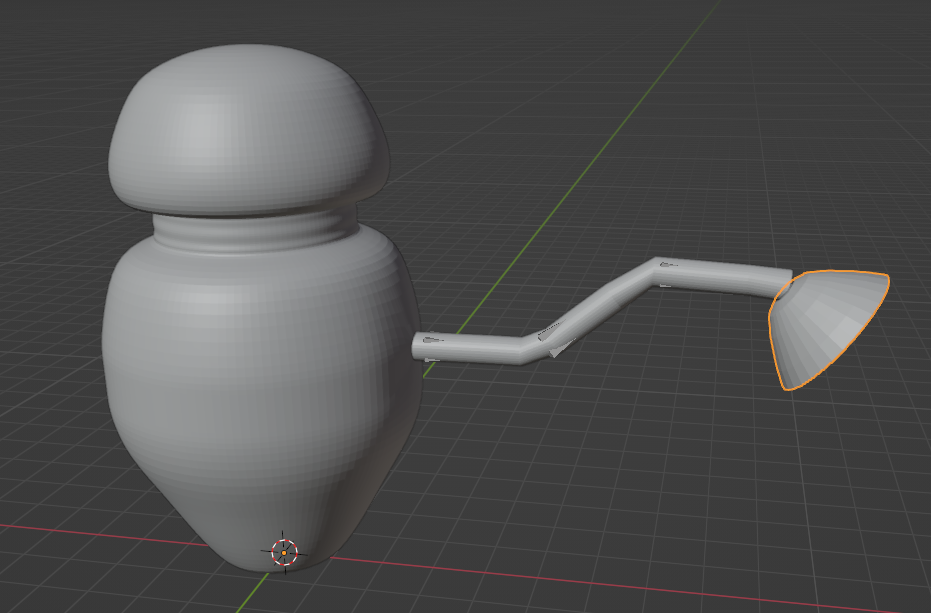
\includegraphics[height=0.3\pageheight,keepaspectratio]{pics/6}
		\caption{Schwebender Roboter}
	\end{subfigure}
	\begin{subfigure}{0.5\textwidth}
		\centering
		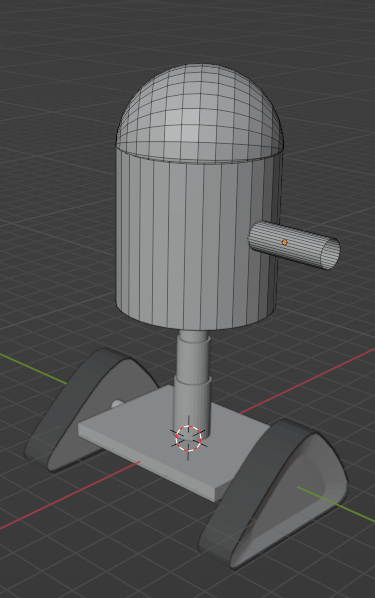
\includegraphics[height=0.3\pageheight,keepaspectratio]{pics/7}
		\caption{Fahrender Roboter}
	\end{subfigure}
	\begin{subfigure}{0.5\textwidth}
		\centering
		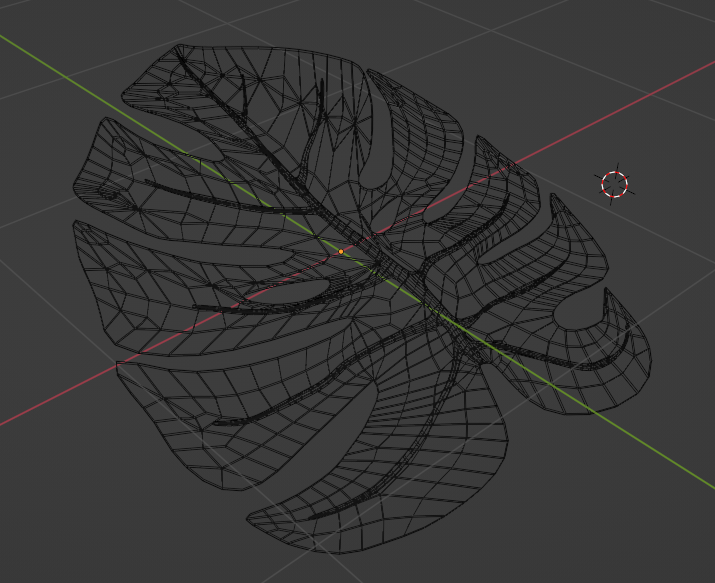
\includegraphics[height=0.3\pageheight,keepaspectratio]{pics/8}
		\caption{Blatt einer Monstera mit zu vielen Polygonen in Wireframedarstellung}
	\end{subfigure}
	\begin{subfigure}{0.5\textwidth}
		\centering
		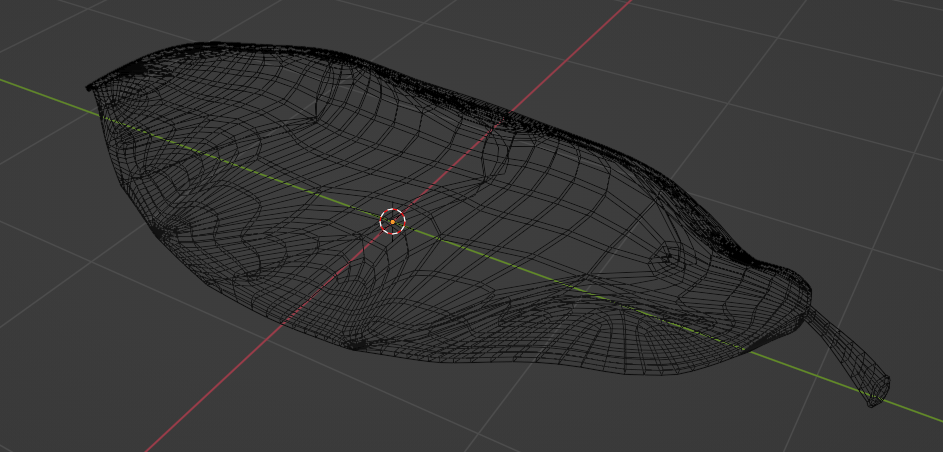
\includegraphics[height=0.3\pageheight,keepaspectratio]{pics/9}
		\caption{Pflanzenblatt mit zu vielen Polygonen in Wireframedarstellung}
	\end{subfigure}
	\caption{Erste Versuche für die Modelle}
\end{figure}
\par
Die Modelle wurden mithilfe von Blender erstellt, während die zugehörigen Texturen eigenständig auf dem iPad mit ProCreate gezeichnet wurden.
\par
Der Roboter wurde primär aus simplen Zylindern modelliert und entsprechend angepasst. Bei der Gestaltung lag der Fokus darauf, dass er ein nicht allzu klassisches Aussehen erhält, da er für Kommunikationszwecke genutzt wird. Die Integration der Solarplatte auf seinem Kopf erfolgte mit der Absicht, dass er sich mittels Sonnenenergie aufladen kann. Der Arm wurde als Schlauch konzipiert, um damit die Pflanzen zu bewässern. Alle einzelnen Objekte wurden bis auf den Schlauch zum Abschluss zu einem einzigen Objekt vereint, während der Schlauch separat blieb, da er später animiert werden soll. In Bezug auf die Texturen wurden bis auf die Solarplatte alle direkt in Blender mithilfe von Geometry Nodes eingestellt. Dadurch erhielt der Körper ein metallisches Aussehen und die Räder einen gummiartigen Look. Die Solarplatte wurde in ProCreate handgezeichnet und anschließend im UV-Editor eingefügt und angepasst. Nach Rücksprache mit dem Team entstand dann unser aktueller Roboter, wie er im MVP zu sehen ist.
\begin{figure}[h]
	\centering
	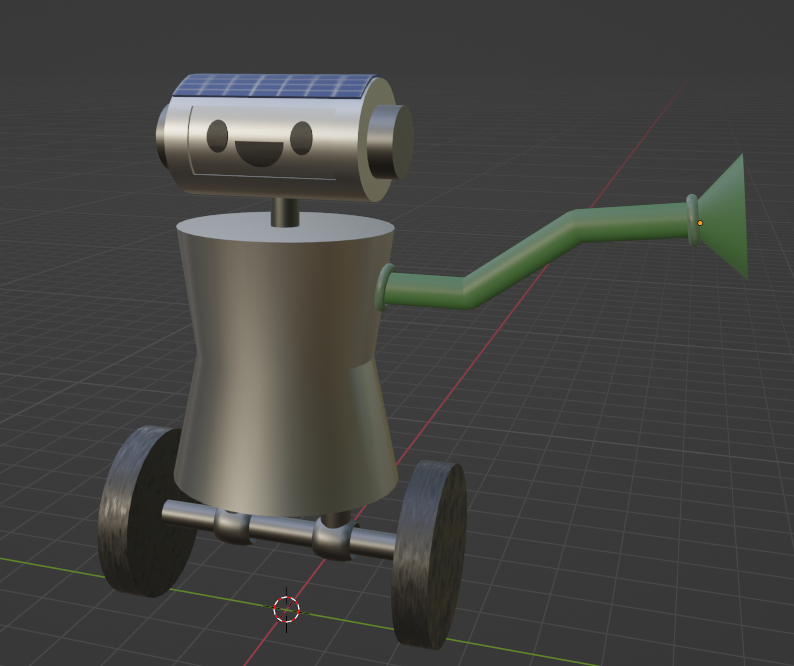
\includegraphics[height=0.3\pageheight,keepaspectratio]{pics/10}
	\caption{Finales Modell für den Roboter}
\end{figure}
\par
Die beiden Pflanzen wurden größtenteils aus spontanen Ideen heraus gestaltet. Die Hauptüberlegung bestand darin, zwei verschiedene Pflanzen zu kreieren. Die Blumentöpfe für beide Pflanzen wurden aus simplen Zylindern modelliert. Ursprünglich wurde der Stiel der kleineren Pflanze mit verschiedenen Einstellungen der Geometry Nodes als komplexes Mesh erstellt. Diese Herangehensweise wurde jedoch verworfen und stattdessen vereinfacht. Die Blätter, die anfangs zu detailliert waren, wurden letztendlich auf zwei einfache 2D-Texturen reduziert. Sowohl die Texturen für die Blätter als auch für die Töpfe mit Erde wurden eigenständig in ProCreate erstellt. Zunächst wurde versucht, die Modelle direkt in ProCreate zu importieren und darauf zu zeichnen. Diese Methode sollte es ermöglichen, die Texturen einfach in Blender zu importieren. Leider funktionierte dieser Ansatz nicht wie erwartet, daher wurden die Texturen schließlich als 2D-Bilder gezeichnet und dann mittels UV-Mapping in Blender angepasst. Ähnlich wie beim Roboter wurden die Pflanzen nach Absprache mit dem Team genehmigt und in das MVP integriert.
\begin{figure}[H]
	\begin{subfigure}{0.5\textwidth}
		\centering
		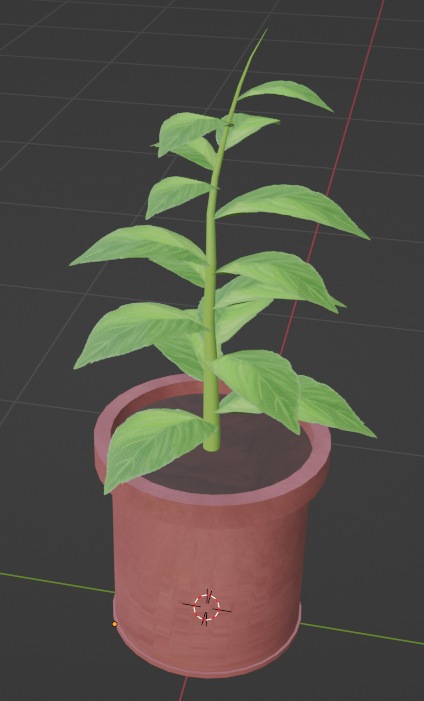
\includegraphics[height=0.3\pageheight,keepaspectratio]{pics/11}
		\caption{Money plant}
	\end{subfigure}
	\begin{subfigure}{0.5\textwidth}
		\centering
		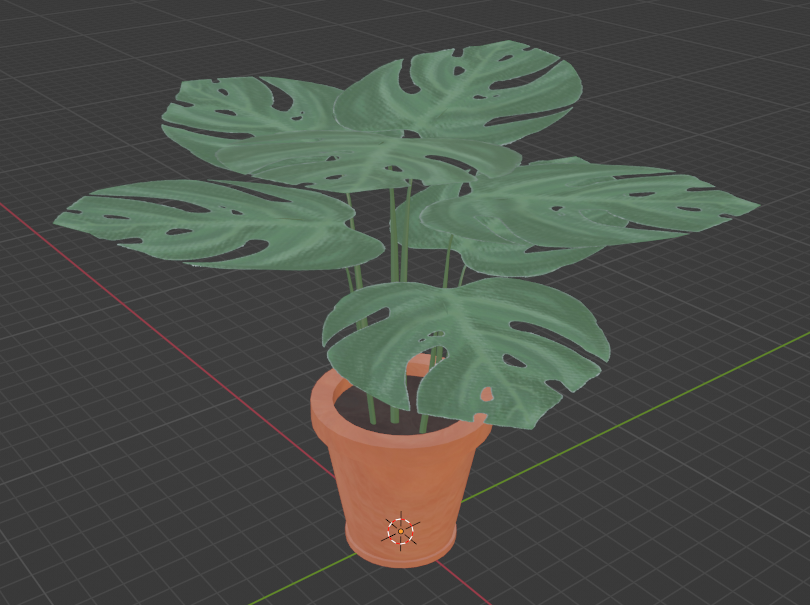
\includegraphics[height=0.3\pageheight,keepaspectratio]{pics/12}
		\caption{Monstera}
	\end{subfigure}
	\caption{Finale Modelle der Pflanzen}
\end{figure}
\par
Die größte Herausforderung lag in der Gestaltung und Implementierung der Plattformen. Wie bereits im Konzept beschrieben, wurden zunächst verschiedene Ansätze dafür entwickelt. Letztendlich wurden beide Plattformen frei nach Gefühl gestaltet, zusammen mit einer etwas unkonventionellen Verbindung zwischen ihnen. Um sicherzustellen, dass die Roboter im Notfall zwischen den Plattformen navigieren können, wurde eine Rampenstruktur um die Säule herum entwickelt. Zusätzlich erhielten sowohl die Rampe als auch die Plattformen Zäune und Geländer, um ihre Sicherheit zu erhöhen. Auch hier wurden alle Texturen eigenhändig mit ProCreate erstellt. Das Modell wurde ebenfalls mit dem Team abgestimmt, bevor es finalisiert wurde.
\begin{figure}[H]
	\centering
	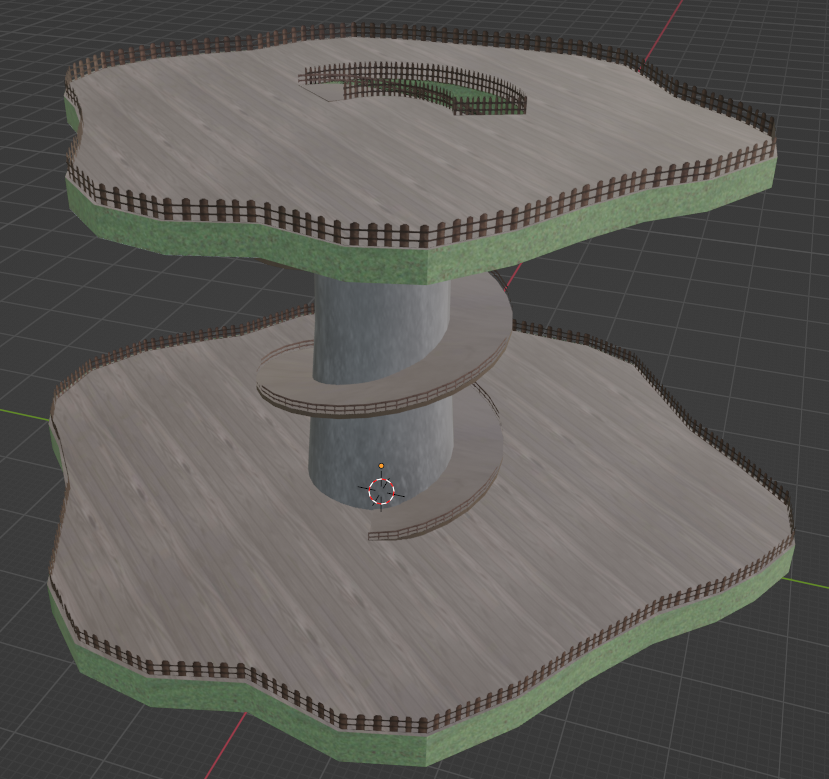
\includegraphics[height=0.3\pageheight,keepaspectratio]{pics/13}
	\caption{Finales Modell der Szene}
\end{figure}
\par
Zum Schluss wurde leider bemerkt, dass die Rampe breiter sein sollte, um Platz für beide Roboter zu bieten, wenn sie gleichzeitig die Ebenen wechseln und sich auf der Rampe treffen. Derzeit gibt es dort keinen Raum zum Ausweichen, was dazu führt, dass einer der Roboter abdriftet.
Nachdem alle Modelle fertiggestellt waren, wurden sie in der Szene zusammengesetzt und weitgehend angepasst. Das gesamte Setup wurde dann mithilfe eines Dropper-Addons in das Projekt integriert. Zunächst gab es einige Probleme und Unklarheiten, die jedoch unter der Leitung des Teamleiters erfolgreich gelöst wurden. Um die Zusammenarbeit zwischen den Modellen und anderen programmatischen Aufgaben wie dem Navigationssystem zu verbessern, wurden die Modelle in "linked" (Pflanzen und Roboter) und "static" (Plattformen \& Co.) unterteilt.
Nachdem die Szene weitgehend fertiggestellt und in das Projekt integriert war, mussten nur noch einige allgemeine Probleme hinsichtlich Texturen und Ordnerstrukturen gelöst werden.
Die nächste Aufgabe bestand darin, die MVP-Szene weiter auszubauen und zu verschönern. Dazu wurden mit Hilfe eines entsprechenden Addons zwei Bäume und ein Haus erstellt. Auch hier wurden alle Texturen für die Bäume und das Haus mit ProCreate erstellt, wobei das Haus noch nicht vollständig fertiggestellt wurde.
\begin{figure}[H]

	\begin{subfigure}{0.5\textwidth}
		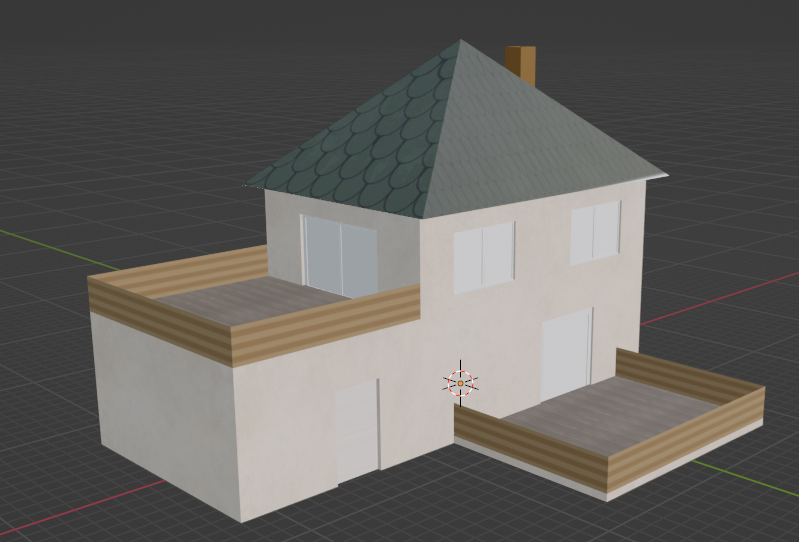
\includegraphics[height=0.3\pageheight,keepaspectratio]{pics/14}
		\caption{Haus mit Terasse}
	\end{subfigure}
	\begin{subfigure}{0.5\textwidth}
		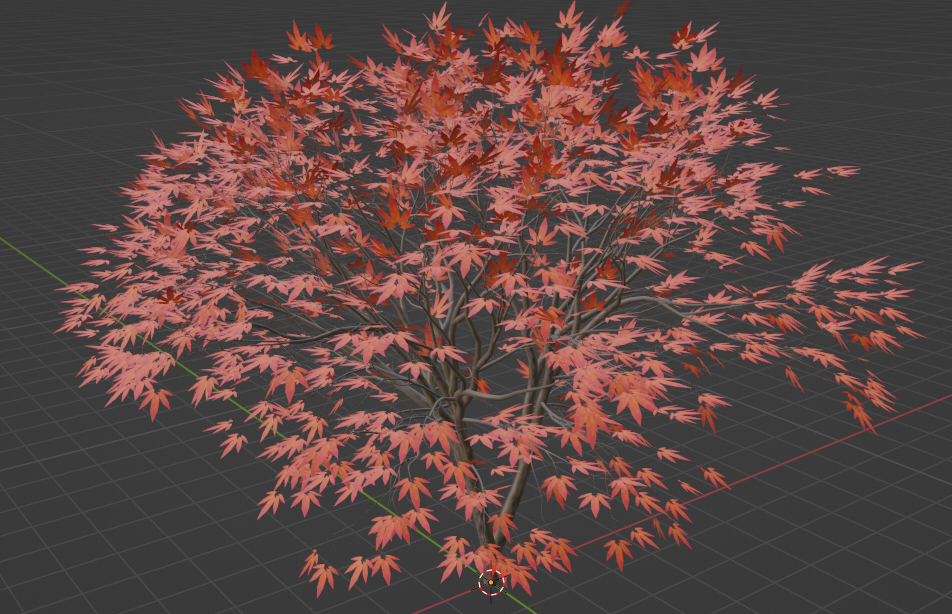
\includegraphics[height=0.3\pageheight,keepaspectratio]{pics/15}
		\caption{Japanischer Ahornbaum}
	\end{subfigure}
	\begin{subfigure}{0.5\textwidth}
		\centering
		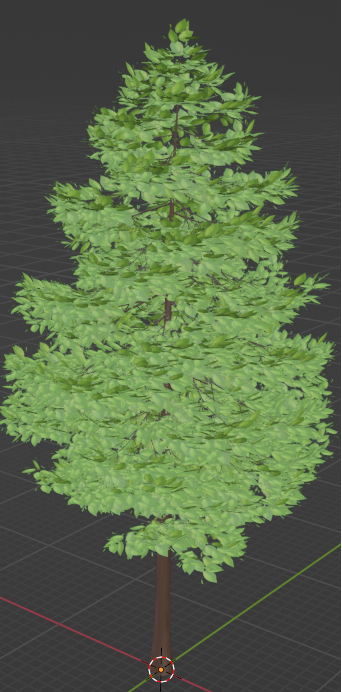
\includegraphics[height=0.3\pageheight,keepaspectratio]{pics/16}
		\caption{Baum}
	\end{subfigure}
	\caption{Modelle für erweiterte Szene}
\end{figure}
\par
Der Ausbau der Szene wurde jedoch vorzeitig beendet, um die verbleibende Zeit dem Bericht zu widmen.